\documentclass{beamer}
\usepackage{beamerthemesplit}
\usetheme{innoQ}
\setbeamertemplate{navigation symbols}{}
% \beamersetuncovermixins{\opaqueness<1>{15}}{\opaqueness<2->{10}}
\usepackage{tikz}
\def\pdfshellescape{1}
\usetikzlibrary{calc}
% \usepackage[utf8]{inputenc}
\usepackage[T1]{fontenc}
\usepackage{textcomp}
% \usepackage{listings}
\usepackage{minted}
\usepackage{graphicx}
\usepackage{wasysym}
\usepackage{url}        % for displaying URLs correctly
\usepackage{soul}       % for \caps
% \usepackage{ulem}       % for \sout
\usepackage{hyperref}
\usepackage[ngerman]{babel}
\usepackage{pifont}

\date{Booster 2013, Bergen, NO \\ 2013-03-14}
\author{FND \& wvk, innoQ Deutschland GmbH}

\title{ROCA}
\subtitle{Embrace the Web}

\definecolor{links}{HTML}{2A1B81}
\hypersetup{colorlinks,linkcolor=,urlcolor=links}

% fonts
\RequirePackage{fontspec}
\defaultfontfeatures{Mapping=tex-text}
\setmainfont[BoldFont={MetaOT-Medi}, BoldItalicFont={MetaOT-MediIta}, ItalicFont={MetaOT-NormIta}, SlantedFont={MetaOT-NormIta}, BoldSlantedFont={MetaOT-MediIta}, Ligatures=TeX]{MetaOT-Norm}
\setsansfont[BoldFont={MetaOT-Medi}, BoldItalicFont={MetaOT-MediIta}, ItalicFont={MetaOT-NormIta}, SlantedFont={MetaOT-NormIta}, BoldSlantedFont={MetaOT-MediIta}, Ligatures=TeX]{MetaOT-Norm}
\newfontfamily\metamedifamily[SlantedFont={MetaOT-MediIta}]{MetaOT-Medi}

% symbol shortcuts for ROCA quiz
\newcommand{\rocaok}{\ding{51}}
\newcommand{\rocafail}{\ding{55}}
\newcommand{\rocastamp}{
  \leavevmode
  \put(220,60){
\includegraphics[width=2.5cm]{images/roca-stamp.png}} %mit \includegraphics ersetzen
}

\begin{document}
  {\usebackgroundtemplate{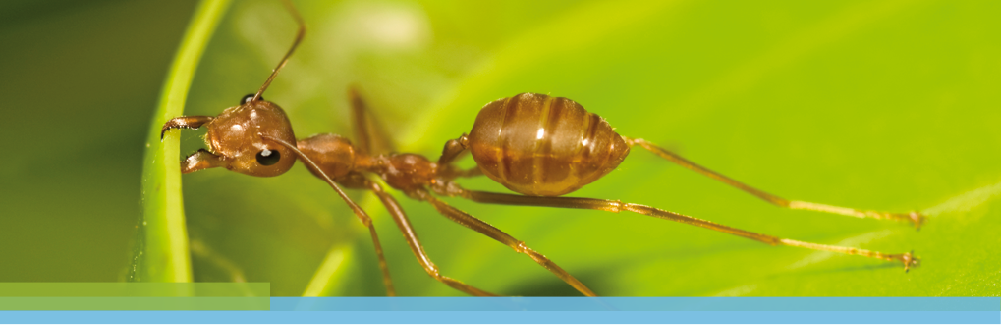
\includegraphics[width=\paperwidth]{images/innoqbg.png}}

  \begin{frame}[plain]
    \titlepage
  \end{frame}
}

\setcounter{tocdepth}{1}

\begin{frame}{Agenda}
  \begin{columns}
    \begin{column}{4.4cm}
      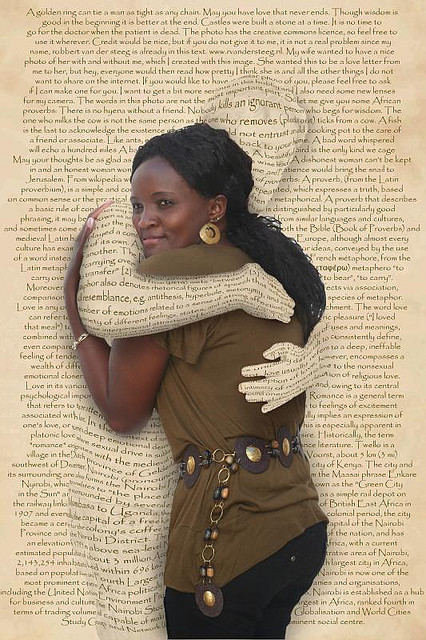
\includegraphics[width=4cm]{images/embrace.jpg}
      \\
      \tiny source: \href{http://www.flickr.com/photos/robbie73/4289385819/}{Robbert van der Steeg}
    \end{column}

    \begin{column}{6.6cm}
      \tableofcontents
    \end{column}
  \end{columns}
\end{frame}

\section{Hej.}

\begin{frame}{\insertsectionhead}
  \begin{itemize}
    \item[FND] Frederik Dohr \href{mailto:fnd@innoq.com}{<fnd@innoq.com>} \\
        recovering SPA enthusiast
    \item[]
    \item[wvk] Willem van Kerkhof \href{mailto:wvk@innoq.com}{<wvk@innoq.com>} \\
        practitioner of others' preachings
  \end{itemize}

  %NOTE general introduction: participants' prior experience & expectations
  %NOTE * technologies (languages & frameworks)
  %NOTE * patterns
  %NOTE * common issues
  %NOTE
  %NOTE /!\ interactivity desired
\end{frame}

\section{What's ROCA?}

{
  \usebackgroundtemplate{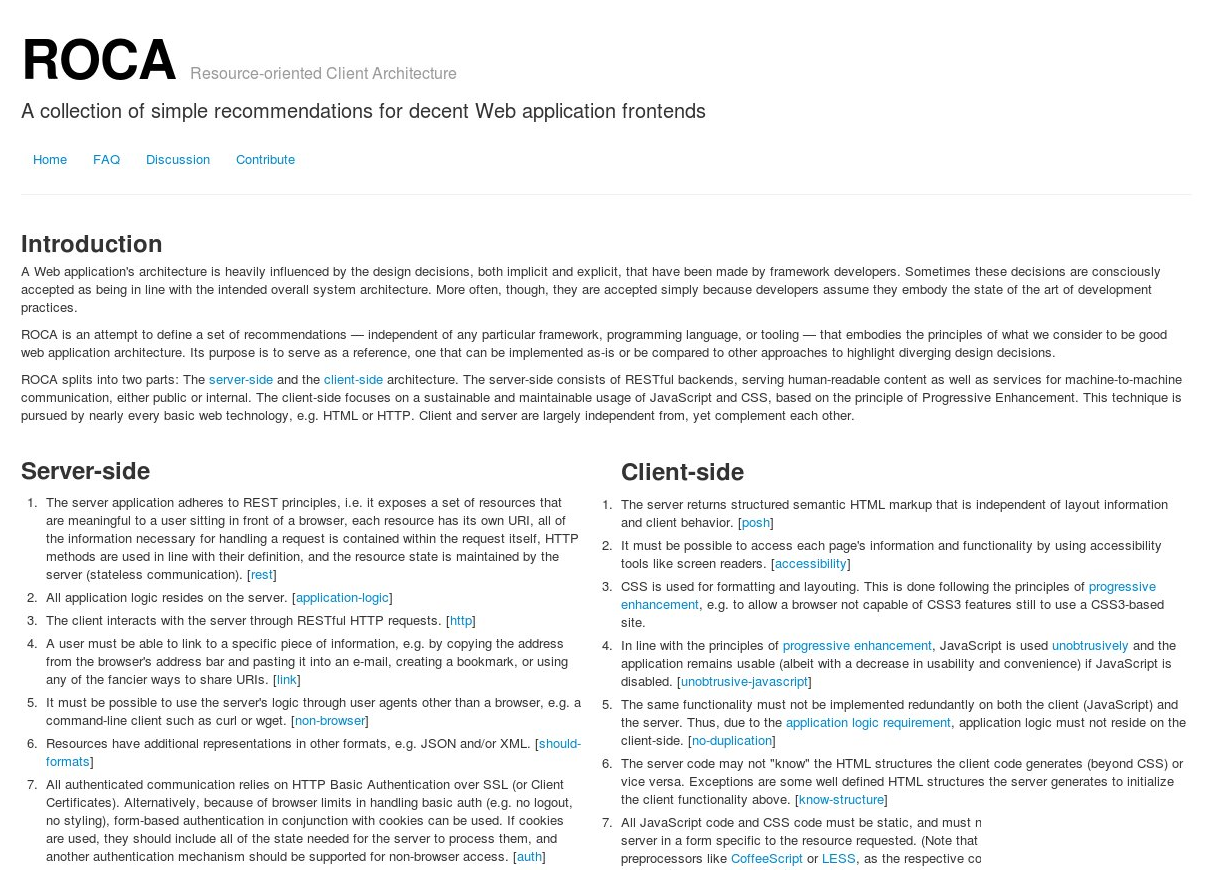
\includegraphics[width=\paperwidth]{images/roca-website.png}}
  \begin{frame}
    \vspace*{-6.4cm}
    \href{http://roca-style.org}{roca-style.org}

    %NOTE proposition for modern, maintainable web apps & the role of the
    %NOTE front-end in particular
  \end{frame}
}

\begin{frame}
  \vspace*{-1cm}
  \textcolor{gray}{
    \begin{center}
      \textbf{
        %FIXME: increase line spacing!
        \fontsize{60}{60}\selectfont Yet another Manifesto?
      }
    \end{center}
  }

  %NOTE * innoQ: consultants - the good kind?
  %NOTE * plethora of possible approaches
  %NOTE * implicit assumptions (often due to frameworks)
  %NOTE * demand for guidance/expertise
\end{frame}

{
  \usebackgroundtemplate{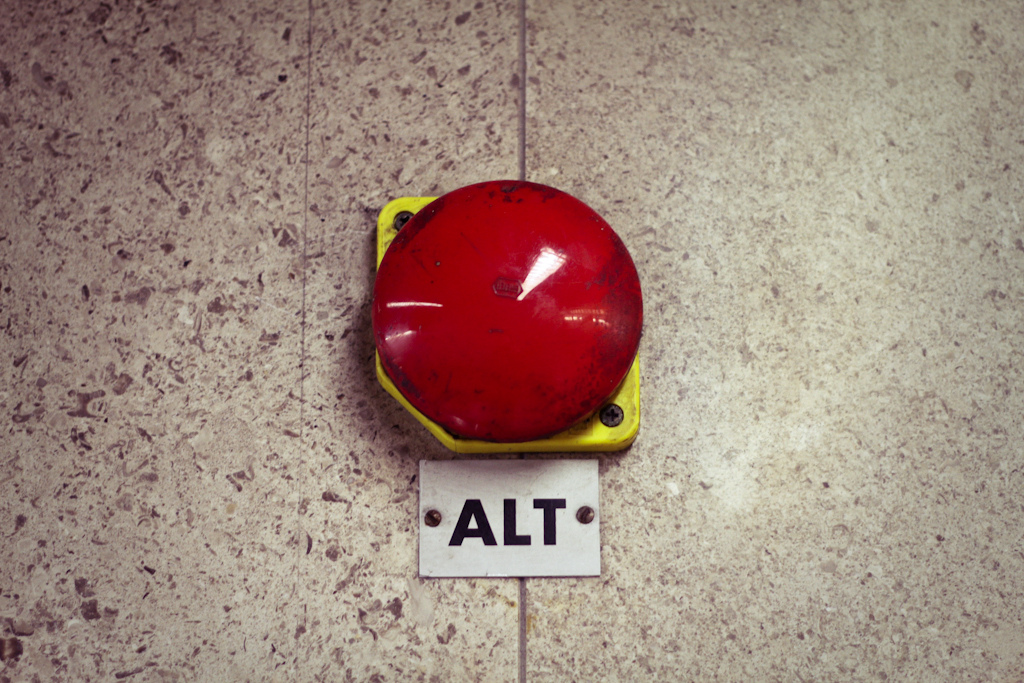
\includegraphics[width=\paperwidth]{images/buzzer.jpg}}
  \begin{frame}
    \vspace*{6.7cm}
    \tiny source: \href{http://www.flickr.com/photos/sensorsicht/5338348801/}{Hannes Fritz}

  %NOTE "label it!"
  %NOTE * makes it referenceable
  %NOTE * triggered discussion
  %NOTE * articulation makes assumptions explicit
  %NOTE
  %NOTE ROCA == set of recommendations to frame architectural discussions
  %NOTE /!\ not scripture - challenge it!
  \end{frame}
}

% TODO: wvk: image with server <---(ROCA)--------->client emphhasis

\begin{frame}[fragile]{\insertsectionhead}
  \textbf{R}esource \textbf{O}riented \textbf{C}lient \textbf{A}rchitecture \dots

  \begin{verbatim}

 server     |<---- ROCA ---->|             client
emphasis ................................ emphasis
  \end{verbatim}

  \dots with server-side emphasis

\end{frame}

\section{Technical Guidelines}

\begin{frame}{Use the Web, Luke}
  \begin{columns}
    \begin{column}{4.0cm}
      
\includegraphics[width=4cm]{images/yoda.png}
      \\
      \tiny source: \href{http://www.flickr.com/photos/barron/15483113/}{Barron Fujimoto}
    \end{column}

    \begin{column}{5.5cm}
      \begin{itemize}
        \item[HTTP] client-server communication
        \item[HTML] content structure
        \item[CSS] presentational aspects
        \item[JavaScript] behavioral augmentation
      \end{itemize}
    \end{column}
  \end{columns}
\end{frame}

\begin{frame}{Meaningful Resources}
  \begin{itemize}
    \item resources represent real or virtual 'things'
    \item resources can be collections
  \end{itemize}
\end{frame}

\begin{frame}
  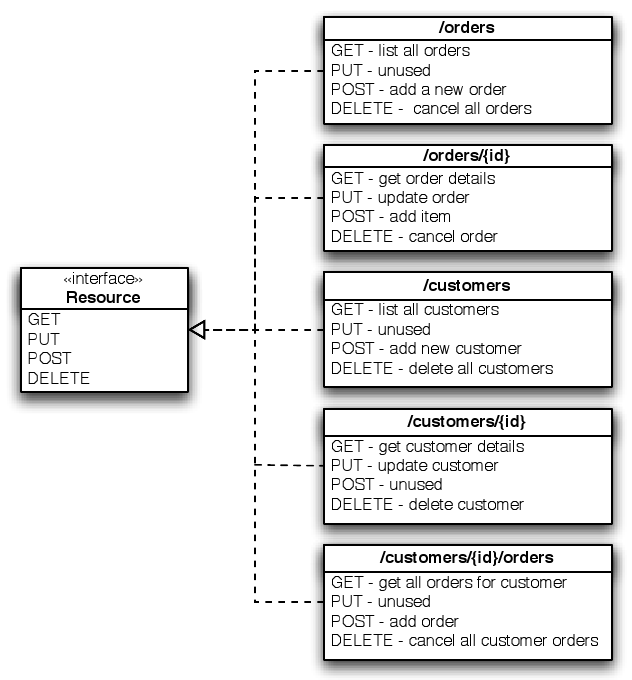
\includegraphics[height=\textheight]{images/rest_example.png}
\end{frame}

\begin{frame}{REST: URIs}
  \begin{itemize}
    \item http://example.com/session
    \item http://example.com/users/fred
    \item http://example.com/users/fred/orders
    \item http://example.com/products?colour=black
    \item https://example.com/processes/money-transfer/new
    \item https://example.com/8e184cc6cf92b8a4725417c56c34a852
  \end{itemize}
\end{frame}

\begin{frame}{REST: Links}
  \begin{itemize}
    \item state transitions via Links (Hypermedia)
    \item traversion of arbitrary associations
    \item links shold be generated by the server, not the client
    \item supports interface evolution
    \item abstracts from absolute locations
  \end{itemize}
\end{frame}

\begin{frame}{REST: HTTP Methods}
  \begin{itemize}
    \item uniform interface for all resources
    \item limited number of HTTP operations (verbs)
    \item pre-defined semantics allows for optimisations (e.g. caching)
  \end{itemize}

  \begin{tabbing}
    {\bfseries HTTP verb} \hspace{0.3cm} \= {\bfseries semantics} \\
    GET    \>  read information, possibly from cache\\
    PUT    \>  update or create with known URI\\
    POST   \>  create sub-resource \\
    DELETE \>  delete, remove (logically)\\
    \dots  \>  \textit{plus a few more.}
  \end{tabbing}
\end{frame}

\begin{frame}{REST: Multiple Representations}
  \begin{itemize}
    \item resource access via representations
    \item possibly multiple representations: HTML, XML, JSON, CSV, \dots
    \item HTTP supports content types and -negotiation
  \end{itemize}
\end{frame}

\begin{frame}{REST: Stateless Communication}

  \begin{itemize}
    \item no need for communication relevant state per client
    \item massive scalability gain
    \item supports loose coupling (communication not bound to a specific server)
  \end{itemize}
\end{frame}

\begin{frame}
  \vspace*{-1cm}
  \textcolor{gray}{
    \begin{center}
      \textbf{
        %FIXME: increase line spacing!
        \fontsize{60}{60}\selectfont Simple as that?
      }
    \end{center}
  }
\end{frame}

\begin{frame}{RESTful HTTP}
  The server application adheres to REST principles

  \begin{itemize}
    \item it exposes meaningful resources
    \item each resource has its own URI
    \item all necessary request handling information is contained within the request
    \item HTTP methods are used in line with their definition
    \item resource state is maintained by the server
  \end{itemize}
  \rocastamp
\end{frame}

\begin{frame}{Cookies}

  Cookies may not be used for purposes other than authentication or user tracking.

  \begin{itemize}
    \item no ``redirect back'' information
    \item no ``flash messages''
    \item no session state
    \item If it's worth persisting, give it a proper server-side resource!
  \end{itemize}
  \rocastamp
\end{frame}

\begin{frame}{Application Logic on Server}
  All essential application logic resides on the server.

  \begin{itemize}
    \item authority \& trust
    \item a service without business logic is a database
  \end{itemize}
  \rocastamp

  %NOTE regarding trust:
  %NOTE * Elster example ("Schnittstelle führt keine Plausibilitätsprüfung durch")
  %NOTE   http://www.golem.de/news/elektronische-steuererklaerung-elster-fuer-linux-und-macos-x-existiert-1303-98024-2.html
\end{frame}

\begin{frame}{No Duplication}

  The same functionality must not be implemented redundantly on both client and server.

  %NOTE Web is linked. Anything non-HTTP ist not cross-linkable (E-mail doesn't count)

  \vspace*{0.25cm}
  \ensuremath{\rightarrow} no application logic on the client (JavaScript)

  \vspace*{0.5cm}
  risks:
  \begin{itemize}
    \item increased maintenance
    \item diverging implementations
    \item subtle differences in interpretation
  \end{itemize}
  \rocastamp
\end{frame}

% FND
\begin{frame}{POSH}
  The server returns structured semantic HTML markup, independent of layout information or client behaviour.\\
  \begin{itemize}
    \item[] NB: alternative serializations are encouraged
  \end{itemize}
  \rocastamp
\end{frame}

% FND
\begin{frame}{HTML}
  \begin{itemize}
    \item constitutes the foundation of the contract between \\ server and client
    \item provides essential data structures with rich, standardized semantics as well as hypermedia support
      \\
      \vspace*{0.25cm}
      \ensuremath{\rightarrow}
      \href{http://codeartisan.blogspot.de/2012/07/using-html-as-media-type-for-your-api.html}{Using HTML as the Media Type for your API}
      \\
      \vspace*{0.25cm}
      \ensuremath{\rightarrow}
      ``lower-case semantic web''
  \end{itemize}
\end{frame}

% FND
\begin{frame}[fragile]
  \frametitle{Extensible Semantics}

  \begin{itemize}
    \item \href{http://microformats.org}{Microformats}
    \item \href{http://www.w3.org/TR/microdata/}{microdata}
    \item \href{http://rdfa.info}{RDFa}
  \end{itemize}

  \begin{minted}{html}
<div class="vcard">
  <span class="fn">Willem van Kerkhof</span>
  <a class="email" href="mailto:wvk@innoq.com">wvk</a>
  <a class="url fn org" href="http://innoq.com">innoQ</a>
</div>
  \end{minted}
  --- \href{http://microformats.org/wiki/hcard}{hCard}

\end{frame}

% FND
\begin{frame}{Unobtrusive JavaScript}
  JavaScript is used unobtrusively

  \begin{itemize}
    \item the application remains usable without JavaScript
    \item usability enhancements and convenience features are added progressively
  \end{itemize}
  \rocastamp
\end{frame}

% FND
\begin{frame}{Unobtrusive JavaScript}
  relying on client-side JavaScript execution is risky

  \begin{itemize}
    \item fault tolerance
    \item transport corruption (e.g. mobile compression)
    \item security filters (e.g. firewalls or browser plugins)
  \end{itemize}
\end{frame}

% FND
\begin{frame}[fragile]
  \frametitle{Unobtrusive JavaScript}

  \begin{itemize}
    \item[]<1|only@1> \begin{minted}{html}
<a href="javascript:doStuff();">action</a>
    \end{minted}
    \item[]<2|only@2> \begin{minted}{html}
<a href="#"
    onclick="doStuff();">action</a>
    \end{minted}
    \item[]<3|only@3> \begin{minted}{html}
<a href="/my-resource"
    onclick="doStuff(this.href);">action</a>
    \end{minted}
    \item[]<4|only@4> \begin{minted}{html}
<a href="/my-resource"
    class="remote">action</a>
    \end{minted}
    \item[]<5|only@5> \begin{minted}{html}
<a href="/my-resource"
    class="remote">action</a>
    \end{minted}
    \vspace*{0.25cm}
    \begin{minted}{javascript}
var elements = document.
        getElementsByClassName("remote");
elements.onclick = function() {
    doStuff(this.href);
};
    \end{minted}
  \end{itemize}
\end{frame}

\begin{frame}[fragile]{Static Assets}
  All JavaScript and CSS code must be static.

  \begin{itemize}
    \item no dynamic per-request code generation
    \begin{minted}{html}
<script>
var message = "hello ${username}";
var element = jQuery("item_${item.id}");
</script>
    \end{minted}
  \end{itemize}

  \begin{columns}
    \begin{column}{8.0cm}
      NB: This does not prohibit the use of preprocessors like LESS \\ or CoffeeScript.
    \end{column}
    \begin{column}{2.5cm}
      \rocastamp
    \end{column}
  \end{columns}
\end{frame}

% FND
\begin{frame}{Progressive Enhancement}
  \vspace*{1cm}
  \center 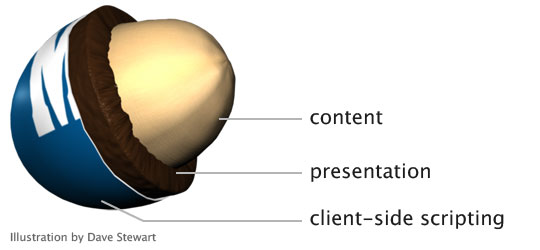
\includegraphics[width=8cm]{images/peanut.jpg}

  \vspace*{1cm}
  \tiny source: \href{http://www.alistapart.com/articles/understandingprogressiveenhancement/}{Understanding Progressive Enhancement}
\end{frame}

\begin{frame}{Progressive Enhancement}

  \begin{exampleblock}{}
    {\large ``A webpage doesn't have to look the same in every browser. In fact, a webpage shouldn't look the same in every browser''}
    \vskip5mm
    \hspace*\fill{\small--- \href{http://www.webmonkey.com/2012/03/video-progressive-enhancement-2-0/}{Nicolas Zakas}}
  \end{exampleblock}

  \vspace*{0.5cm}
  offering users the best possible experience \\
  given the capabilities of their device
\end{frame}

% FND
{
  \usebackgroundtemplate{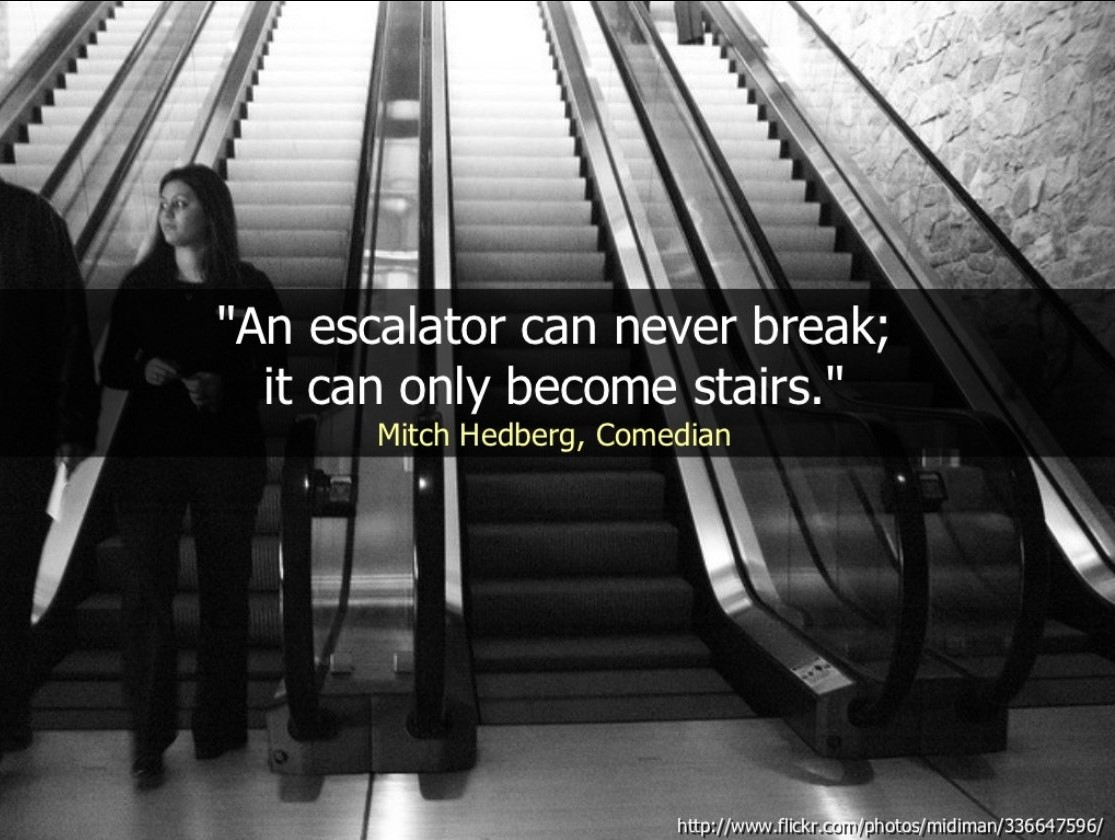
\includegraphics[width=\paperwidth]{images/escalator.jpg}}
  \begin{frame}
    \vspace*{6.7cm}
    \textcolor{gray}{\tiny
        sources:
        \href{http://www.flickr.com/photos/midiman/336647596}{midiman},
        \href{http://www.slideshare.net/nzakas/progressive-enhancement-20-conference-agnostic}{Nicolas Zakas}
    }
  \end{frame}
}

% FND
\begin{frame}[fragile]{Progressive Enhancement}

  \begin{minted}[fontsize=\footnotesize]{html}
<div class="tabs">
    <ul>
        <li> <a href="#about">About</a> </li>
        <li> <a href="#toc">Table of Contents</a> </li>
        <li> <a href="#comments">Discussion</a> </li>
    </ul>

    <p id="about">lorem ipsum dolor sit amet</p>
    <ol id="toc"> ... </ol>
    <div id="comments"> ... </div>
</div>
  \end{minted}
  \begin{minted}[fontsize=\footnotesize]{javascript}
jQuery(".tabs").tabs();
  \end{minted}

  \tiny \ensuremath{\rightarrow} \href{http://jqueryui.com/tabs/}{jQuery UI}
\end{frame}

% FND
\begin{frame}[fragile]
  \frametitle{Progressive Enhancement}

  \begin{minted}{html}
    <input type="date">
  \end{minted}
  \begin{minted}{javascript}
    jQuery("input[type=date]").datepicker();
  \end{minted}

  \vspace*{0.5cm}
  \begin{minted}{html}
    <table class="sortable">
        ...
    </table>
  \end{minted}
  \begin{minted}{javascript}
    jQuery("table.sortable").dataTable();
  \end{minted}
\end{frame}

% FND
\begin{frame}{Progressive Enhancement}
  \begin{itemize}
    \item separation of concerns \\ encapsulation, loose coupling
    \item maintainability \& reusability
  \end{itemize}
  \rocastamp

  \vspace*{-0.5cm}
  \ensuremath{\rightarrow}
  \href{http://helloworld.innoq.com/workshops/javascript/part4.html\#slide-40}{component lifecycle}
\end{frame}

\section{UX Consequences}

\begin{frame}
  \vspace*{-1cm}
  \textcolor{gray}{
    \begin{center}
      \textbf{
        \fontsize{60}{50}\selectfont \insertsectionhead
      }
    \end{center}
  }
\end{frame}

\begin{frame}{Links}
  A user must be able to link to a specific piece of information

  \begin{itemize}
    \item e.g. by copying the address from the browser's address bar
    \item pasting it into an e-mail or IM
    \item creating a bookmark
    \item or using any of the fancier ways to share URIs
  \end{itemize}
  \rocastamp
\end{frame}

\begin{frame}{Non-Browser Clients}
  The server's logic should be accessible to user clients other than a web browser.

  \begin{itemize}
    \item crawler, indexer (SEO for free, yay!)
    \item alternative user agent (curl, text browser, screen reader etc.)
    \item arbitrary unanticipated usage
  \end{itemize}

  \rocastamp
\end{frame}

\begin{frame}{Formats}
  Resources have additional representations in other formats.

  \begin{itemize}
    \item e.g. JSON, XML, CSV (read/write)
    \item \dots or PDF or XLSX reports (read-only)
  \end{itemize}
  \rocastamp
\end{frame}

\begin{frame}{Browser Controls}

  The browser controls like the back, forward and refresh buttons must work as expected.

  \begin{itemize}
    \item[back] \ensuremath{\rightarrow} user's last meaningful resource
    \item[refresh] \ensuremath{\rightarrow} no re-rendering of the login or home page
    \item mind the the POST verb!
  \end{itemize}
  \rocastamp
\end{frame}

\begin{frame}{Accessability}

  Each page's information and functionality must be accessible by tools like screen readers.

  \begin{description}
    \item[keyboard shortcuts:] fine, but not everyone uses a keyboard
    \item[pointing devices:] likewise
  \end{description}

  \rocastamp
\end{frame}

\section{Quiz Time!}

\begin{frame}
  \vspace*{-1cm}
  \textcolor{gray}{
    \begin{center}
      \textbf{
        \fontsize{50}{50}\selectfont It's your turn.
      }
    \end{center}
  }
\end{frame}

\begin{frame}{\insertsectionhead}
  \vspace*{0.5in}

  \begin{columns}
    \begin{column}{2.2cm}
    \end{column}

    \begin{column}{2.2cm}
      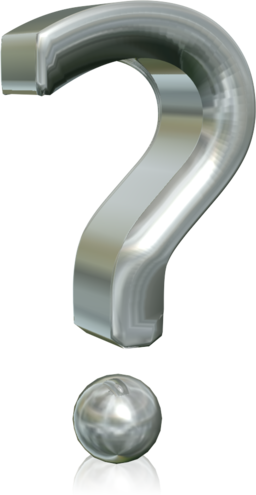
\includegraphics[width=2cm]{images/quiz.png}
    \end{column}

    \begin{column}{6.6cm}
      ROCA or not
      \vspace{0.3cm}
      \begin{itemize}
        \item[$\square$] \rocaok
        \item[$\square$] \rocafail
      \end{itemize}
    \end{column}
  \end{columns}

  \vspace*{0.4in}
  \tiny source: \href{http://commons.wikimedia.org/wiki/File:Question_mark_3d.png}{Hay Kranen}
\end{frame}

\begin{frame}
  When sharing a URL with another user, that user is presented with an empty page.

  \vspace{0.3cm}
  \begin{itemize}
    \item<1|only@1>[\Large $\square$] \Large ROCA?
    \item<2|only@2>[\Large \rocafail] \Large ROCA?
    \item<2> session state?
    \item<2> JavaScript problem?
    \item<2> hashbang URIs?
  \end{itemize}

  %NOTE e.g. due to JavaScript errors (cf. Gawker hashbang URIs)
  %NOTE e.g. due to session state
\end{frame}

\begin{frame}
  When refreshing the page, the user is taken to the respective site's front page.

  \vspace{0.3cm}
  \begin{itemize}
    \item<1|only@1>[\Large $\square$] \Large ROCA?
    \item<2|only@2>[\Large \rocafail] \Large ROCA?
    \item<2> client-side logic?
    \item<2> HTML5 history API?
    \item<2> where's the REST?
  \end{itemize}

  %NOTE URI/resource violation (e.g. bookmarks, sharing)
\end{frame}

\begin{frame}
  After using the browser's back button, the user is presented with an error
  messsage informing them to use the website's own navigation controls instead.

  \vspace{0.3cm}
  \begin{itemize}
    \item<1|only@1>[\Large $\square$] \Large ROCA?
    \item<2|only@2>[\Large \rocafail] \Large ROCA?
    \item<2> where's the REST?
    \item<2> there should be no difference between linking, sharing and history navigation
  \end{itemize}

  %NOTE URI/resource violation
\end{frame}

\begin{frame}
  Shortly after starting a booking process for a train journey, the user is
  interrupted and returns several minutes later to complete his booking. Filling
  out and submitting the form, he is presented with a session timeout message.

  \vspace{0.3cm}
  \begin{itemize}
    \item<1|only@1>[\Large $\square$] \Large ROCA?
    \item<2|only@2>[\Large \rocafail] \Large ROCA?
    \item<2> Session state on server?
  \end{itemize}

  %NOTE REST stateless violation
\end{frame}

\begin{frame}
  On a slow connection, ads, navigation elements, footers and other secondary
  information are slowly displayed first. Eventually, the main content is displayed.

  \vspace{0.3cm}
  \begin{itemize}
    \item<1|only@1>[\Large $\square$] \Large ROCA?
    \item<2|only@2>[\Large ?] \Large ROCA?
    \item<2> not a ROCA validation (but still annoying)
    \item<2> ``content first''
  \end{itemize}

  %NOTE POSH violation? not strictly
\end{frame}

\begin{frame}
  Dashboard contents are loaded asynchronously via AJAX.

  \vspace{0.3cm}
  \begin{itemize}
    \item<1|only@1>[\Large $\square$] \Large ROCA?
    \item<2|only@2>[\Large \rocaok] \Large ROCA?
    \item<2> Progressive Enhancement from simple links \\ (\ensuremath{\rightarrow} hypermedia)
  \end{itemize}

  %NOTE fine - as long as it's POSH-based
\end{frame}

\begin{frame}
  When refreshing a page displaying search results, the browser prompts the
  user to confirm whether they really want to submit the form again.

  \vspace{0.3cm}
  \begin{itemize}
    \item<1|only@1>[\Large $\square$] \Large ROCA?
    \item<2|only@2>[\Large \rocafail] \Large ROCA?
    \item<2> mind the POST verb!
  \end{itemize}

  %NOTE REST verb violation
\end{frame}

\begin{frame}
  Comments are loaded asynchronously after the page has loaded.

  \vspace{0.3cm}
  \begin{itemize}
    \item<1|only@1>[\Large $\square$] \Large ROCA?
    \item<2|only@2>[\Large \rocaok] \Large ROCA?
    \item<2> depends on implementation
    \item<2> link to comments?
  \end{itemize}

  %NOTE depends on the implementation: Disqus bad, link good
\end{frame}

\begin{frame}
  The current page's JavaScript source code is minified and obscured, thus hard
  to read.

  \vspace{0.3cm}
  \begin{itemize}
    \item<1|only@1>[\Large $\square$] \Large ROCA?
    \item<2|only@2>[\Large \rocaok] \Large ROCA?
  \end{itemize}

  %NOTE fine (sadly)
\end{frame}

\begin{frame}
  After clicking the ``proceeed with secure payment'' link, a browser popup window
  warns about an untrusted SSL certificate. After confirming its trust, a second
  popup asks for the user's login credentials.

  \vspace{0.3cm}
  \begin{itemize}
    \item<1|only@1>[\Large $\square$] \Large ROCA?
    \item<2|only@2>[\Large \rocaok] \Large ROCA?
    \item<2> HTTP basic auth over SSL, perfect.
    \item<2> wanna talk about trusted CAs?
  \end{itemize}

  %NOTE perfect, especially for intranet stuff. for public sites, see next slide.
\end{frame}

\begin{frame}
  Because of browser limitations in handling basic auth (e.g. no logout, no styling),
  form-based authentication in conjunction with cookies is being used.

  \vspace{0.3cm}
  \begin{itemize}
    \item<1|only@1>[\Large $\square$] \Large ROCA?
    \item<2|only@2>[\Large \rocaok] \Large ROCA?
    \item<2> OK, if all necessary state information is stored in the cookie.
    \item<2> Basic auth for non-browser clients
  \end{itemize}

  %NOTE fine, but if cookies are used, they should include all of the state needed for
  %NOTE the server to process them, and another authentication mechanism should be
  %NOTE supported for non-browser access
\end{frame}

\begin{frame}
  Inpecting the current page's source code reveals a minimal HTML frame with
  JSON data embedded in a \texttt{<SCRIPT>} tag.

  \vspace{0.3cm}
  \begin{itemize}
    \item<1|only@1>[\Large $\square$] \Large ROCA?
    \item<2|only@2>[\Large \rocafail] \Large ROCA?
    \item<2> think POSH!
    \item<2> think Progressive Enhancement!
  \end{itemize}

  %NOTE JavaScript dependency violation (cf. Google Plus)
\end{frame}

\begin{frame}[fragile]
  Selecting ``open link in new tab'' results in a blank page.

  \vspace{0.3cm}
  \begin{itemize}
    \item<1|only@1>[\Large $\square$] \Large ROCA?
    \item<2|only@2>[\Large \rocafail] \Large ROCA?
    \item<2> bad: \mint{html}|<a href="javascript:...;">|
    \item<2> different, yet still bad: \mint{html}|<a href="#">|
  \end{itemize}
\end{frame}

\begin{frame}
  Form inputs from a previous step are stored in cookies to be retrieved by
  JavaScript for validations in the next step.

  \vspace{0.3cm}
  \begin{itemize}
    \item<1|only@1>[\Large $\square$] \Large ROCA?
    \item<2->[\Large \rocafail] \Large ROCA?
    \item<2-> Session state?
    \item<2-> Application logic on Client?
    \item<3> think of a better solution?
  \end{itemize}

  %NOTE e.g. a multi-step wizard.
\end{frame}

\begin{frame}
  Opening the current page in a second browser window renders the first page inoperable.

  \vspace{0.3cm}
  \begin{itemize}
    \item<1|only@1>[\Large $\square$] \Large ROCA?
    \item<2->[\Large \rocafail] \Large ROCA?
    \item<2-> session state
  \end{itemize}

\end{frame}

\begin{frame}
  \vspace*{-2cm}
  \textcolor{gray}{
    \begin{center}
      \textbf{ \fontsize{50}{80} \selectfont You did well. \\ }
      {\fontsize{30}{30} \selectfont Thank you!}
    \end{center}
  }
\end{frame}

\begin{frame}{Key Takeaways}
  \begin{itemize}
    \item RESTful HTTP
    \item server-side authority
    \item POSH
    \item unobtrusive JavaScript
    \item no duplication
  \end{itemize}
\end{frame}

\begin{frame}{ROCAful Examples}
  \begin{itemize}
    \item \href{http://fnd.github.com/hijax-demo/}{Hijax demo}
    \item \href{http://pjax.heroku.com}{pjax}
    \item \href{https://github.com/rails/turbolinks}{Turbolinks}
    \item \href{http://rocatodo.herokuapp.com}{TodoMVC (ROCA)}
  \end{itemize}
\end{frame}

\begin{frame}{Contact}
  \begin{columns}
    \column{5cm}
    
\includegraphics[width=4cm]{images/innoQ-Logo-RGB-72dpi.png}
    \vspace{4mm}
    \column{4.5cm}

    \href{http://www.innoq.com}{http://www.innoq.com} \\
    \href{mailto:info@innoq.com}{info@innoq.com}
  \end{columns}

  innoQ Deutschland GmbH \\
  Krischerstraße 100 \\
  D-40789 Monheim \\
  Tel (+49) 2173 3366 0
\end{frame}

\end{document}
